\section{The Software Out-of-Order Processor}
\label{sec:soop}

Legion uses a {\em  software out-of-order processor}, or SOOP, to schedule tasks.  A SOOP 
dynamically schedules a stream of tasks in a manner akin to an out-of-order processor scheduling a stream of instructions:
just as an instruction scheduler is constrained by register dependences,
the SOOP is constrained by region dependences.
The SOOP  is pipelined, distributed and extracts nested parallelism from subtasks.
There are two major challenges in implementing an efficient task scheduler:
\begin{itemize}
\item  For correctness, Legion must preserve data dependences between tasks, which is non-trivial
because the same data may be in multiple different regions or subregions.
  
\item For performance, Legion must hide the extremely long latencies associated
  with machines that have both distributed memory and many levels of
  memory hierarchy.
\end{itemize}

To solve the second problem Legion uses a {\em deferred execution model} that decouples the issuing
of operations from when operations are performed.  Using a low-level runtime event system (which we do
not describe further in this paper), an issued operation waits for other operations on
which it is dependent to complete before executing, but a waiting operation does not cause the SOOP
to block.  With deferred execution, it is worthwhile for the SOOP to run (potentially far) ahead of actual execution,
allocating resources to and issuing tasks that must wait because they have data dependences on earlier tasks that have not 
finished executing.   Pipelining and distributing the SOOP further improves throughput and hides latency.

To dynamically detect and enforce data dependences,
the SOOP considers, for each task $t$, the
the regions $t$ uses and ensures $t$ waits on any
earlier task whose region uses conflict with $t$'s.  There is a
difficulty, however.  The programmer's regions are logical; a region
names a set of objects, but does not say where those objects
are in memory.  To ensure dependences are satisfied the SOOP must also {\em map} $t$: assign an
appropriate physical instance to each of $t$'s logical regions.  Thus, dependence
analysis requires knowing both which tasks $t$ depends on and how those
other tasks are mapped.

Our SOOP design solves this problem by dividing the analysis of
dependences between two pipeline stages.  The first SOOP stage
computes task dependences at the granularity of logical regions
(Section~\ref{sec:dep}), which does not give enough information to map
$t$, but does identify all tasks that must map before $t$ can map.
The third SOOP stage maps $t$ by carrying out a more refined analysis
of the (already mapped) tasks on which $t$ depends
(Section~\ref{sec:map}).  Between these stages, the second stage
distributes tasks to other processors (Section~\ref{sec:dist}).  Once
a task has been assigned a processor and physical instances it is
issued for deferred execution (Section~\ref{sec:exec}).  The final
SOOP stage reclaims resources from completed tasks
(Section~\ref{sec:clean}).

\subsection{Stage 1: Mapping Dependences}
\label{sec:dep}


%When a Legion task runs, it may spawn new subtasks to be executed.  
%These subtasks are {\em children} of the {\em parent} task and {\em siblings} of each other.  
%A task always executes on a single processor, but
%its subtasks may execute elsewhere.

Each processor in the system runs an instance of the SOOP.
When a {\em parent} task spawns a {\em child} task, the child is {\em registered}
with the SOOP on the parent's processor;
registration records the subtask's logical regions,
privileges and coherence properties.  Children are
registered in the sequential order the parent
spawns them and enqueued for mapping dependence analysis.  In the
circuit simulation in Listing~\ref{lst:code_ex}, the spawn
statements on lines 32-34 register all three
kinds of subtasks (in program order) on the processor where {\tt
simulate\_circuit} executes.

Detecting mapping dependences between a newly registered task $t$ and
a previously registered task $t'$ requires comparing the two sets of
logical regions accessed.  For each logical region used by $t'$ that
may {\em alias} (may share data with) a logical region used by $t$, the privileges and
coherence modes are compared to determine whether a dependence exists.
If both regions need only read privileges there is never a dependence,
but if either task needs write or reduction privileges, the coherence
modes are compared using the table in Figure~\ref{fig:dependence}.
{\tt Dep} indicates dependence while {\tt None}
indicates independence.  {\tt Same} is a dependence unless the two tasks
use the same physical instance of the logical region.
%\footnote{For example, if two tasks wish to acess the region with atomic coherence, then if they are working on the same physical copy of the data atomicity can be guaranteed using, e.g., locking.  If they are working on different copies of the data then the only safe execution strategy for Legion is to serialize the two tasks.}
{\tt Cont} 
indicates a dependence unless a single writer has
atomic coherence.  


\begin{figure}
{\small
\begin{tabular}{c|cccc}
             & Exclusive & Atomic   & Simultaneous & Relaxed \\
\midrule
Exclusive    & Dep & Dep & Dep & Dep \\ 
Atomic       & Dep & Same & Cont & Cont \\
Simultaneous & Dep & Cont & Same & None \\
Relaxed      & Dep & Cont & None & None \\
\end{tabular}
}
\caption{Dependence table.}
\label{fig:dependence}
\end{figure}

The table lists {\em simultaneous} and {\em relaxed} coherence modes
that we have not yet discussed.  Both modes
allow other tasks using the region to execute at the same time and differ
only in what updates must be observed.  With simultaneous coherence, a task must 
see all updates to the logical region made by other tasks operating on the same region 
simultaneously (i.e., shared memory semantics).  With relaxed coherence, 
a task may or may not observe concurrent updates.


%
%\begin{figure}
%
%\centering
%\begin{tikzpicture}
%\node(top) at (3.5,3.5) { $p$ };
%
%\node(s1) at (1.9,2.5) { $s1$ };
%\node(s2) at (5.1,2.5) { $s2$ };
%
%\node(m1) at (1.9,1.5) { $\ldots$ };
%\node(m2) at (5.1,1.5) { $\ldots$ };
%\node(t1) at (1.9,0.5) { $t_1$ };
%\node(t2) at (5.1,0.5) { $t_2$ };
%
%\draw
%  (top.south) edge (s1.north)
%  (s2.north) edge (top.south)
%  (m1.north) edge (s1.south)
%  (m2.north) edge (s2.south)
%  (t1.north) edge (m1.south)
%  (t2.north) edge (m2.south)
%  ;
%
%\draw[dashed]
%  (t1.east) edge (t2.west)
%  (s1.east) edge (s2.west)
%  ;
%
%\end{tikzpicture}
%\caption{Dependence between tasks implies a dependence between siblings of the least common ancestor.}
%\label{fig:independence}
%\end{figure}

A key property of Legion is that dependence analysis is only needed
between sibling tasks:
\begin{observation}
\label{obs:isolation}
\rm
Let $t_1$ and $t_2$ be two sibling tasks with no dependence.  Then no subtask of $t_1$ has a dependence with any subtask
of $t_2$.
\end{observation}
Recall from Section~\ref{sec:ex} that subtasks only access subregions of their parent task's region arguments (and with fewer
privileges).  Thus if the regions used by $t_1$ and $t_2$ do not alias, the regions used by any subtasks of $t_1$ cannot
alias the regions used by any subtask of $t_2$.  If the regions used by $t_1$ and $t_2$ alias
but there is no dependence because the regions are used with simultaneous or relaxed coherence, then by definition there is no dependence between the subtasks.

Consider the first two subtasks spawned on line 32 of the circuit
simulation in Listing~\ref{lst:code_ex}, {\tt
calc\_new\_currents(pieces[0])} and {\tt
calc\_new\_currents(pieces[1])}.  The first of these tasks reads and
writes the private wires subregion {\tt pieces[0].rw\_pvt} in
exclusive mode, and reads in exclusive mode the node subregions {\tt
pieces[0].rn\_pvt}, {\tt .rn\_shr}, and {\tt
.rn\_ghost} (see line 39).  The second subtask must be
checked against the first for any dependences; the second subtask uses
{\tt pieces[1].rw\_pvt} (read/write exclusive) and {\tt
pieces[1].rn\_pvt}, {\tt .rn\_shr}, and {\tt .rn\_ghost} (read-only exclusive).
It may be helpful to refer to the region tree for nodes in Figure~\ref{sfig:part_fig:tree} (recall that the wires region tree consists of a single disjoint partition).  We give a few representative examples
of reasoning about pairwise dependences (not all pairs are covered):
\begin{enumerate}
\item {\tt pieces[0].rw\_pvt} and {\tt pieces[1].rw\_pvt} do not alias as they are subregions of a disjoint partition.
%\item {\tt pieces[0].rn\_pvt} and {\tt pieces[1].rn\_pvt} do not alias for the same reason.
%\item {\tt pieces[0].rn\_shr} and {\tt pieces[1].rn\_shr} do not alias, also for the same reason.
\item {\tt pieces[0].rn\_ghost} aliases {\tt pieces[1].rn\_shr}, because they are in two different
  partitions of the same region.
%\item {\tt pieces[0].rn\_shr} and {\tt pieces[1].rn\_ghost} alias because they are in two different
  partitions of the same region.
\item {\tt pieces[0].rn\_ghost} aliases {\tt pieces[1].rn\_ghost} because they are in different subregions of
an aliased partition.
\item {\tt pieces[0].rw\_pvt} and {\tt pieces[1].rn\_pvt})
do not alias because they are in different region trees and have no common region ancestor.
\end{enumerate}
Cases 2 and 3 indicate a possible dependence, however the regions are
accessed with only read privileges. All other cases for these two
subtasks are similar to one of the examples above; thus, the two
subtasks are independent.

A closer look at this example shows that whether there is aliasing
between two regions $r_1$ and $r_2$ can be determined by examining
their least common ancestor $\lca{r_1}{r_2}$ in the region tree.  
There are four cases.  If $\lca{r_1}{r_2}$ either does not exist (the regions
are in different region trees) or is a disjoint partition, then $r_1$
and $r_2$ are disjoint.  If $\lca{r_1}{r_2}$ is an
aliased partition or a region, 
%(because $r_1$ and $r_2$ are in
%different partitions of the region, as in cases 4 and 5
%above), 
then $r_1$ and $r_2$ may not be disjoint.

Consider tasks {\tt distribute\_charge(pieces[0],dt)} and
{\tt update\_voltages[1]} in Listing~\ref{lst:code_ex}.  The former task
uses region {\tt pieces[0].rn\_ghost} and the latter uses region {\tt pieces[1].rn\_shr}.
The least common ancestor is the region of all shared nodes {\tt p\_nodes\_pvs[1]},
so these two regions are not disjoint.  Since both tasks write their respective subregions,
there is a dependence and the {\tt update\_voltages} task can only map after the
{\tt distribute\_charges} task has mapped.

We can now describe the algorithm for the dependence analysis phase of
the SOOP.  The SOOP maintains a local region forest for each task $t$,
the roots of which are $t$'s region arguments and including all
partitions and subregions used by $t$.  Dependence analysis
places the child tasks of $t$ on the regions they use, maintaining the
following invariant. Let $r'$ be a region used by child task $t'$,
and let $R$ be the set of regions $r''$ such that $r''$ is used
by a task $t''$ registered after $t'$ and $t''$ depends on $t'$
because of aliasing between $r''$ and $r'$.  Then $t'$ is listed on the
region that is the least common ancestor of the set $R \cup \{r'\}$.
Placing $t'$ on an ancestor of $r'$ has the effect of coarsening the
dependences involving $t'$, which
can result in false dependences.  However, the loss of
information can be shown to be small and only affects when $t$ can
map; any information lost is recovered during mapping.
Furthermore, the benefit is that it dramatically speeds up
dependence analysis overall.

We can identify all mapping dependences between sibling tasks and place tasks
in the correct place in the region tree in amortized time ${\cal O}(d)$ per region,
where $d$ is the depth of the region tree.  For region $r'$ an argument of task $t'$, the analysis
walks the unique path in the region forest from a root to $r'$.  For each node $m$
on the walk from the root to $r'$ the following actions are taken:
\begin{itemize}
\item If $m$ is a region with multiple child partitions and $m'$ is the child on the
path to $r'$, then any task in a subtree of $m$ other than $m'$ on which $t'$ depends 
is moved to $m$.

\item If $m$ is a non-disjoint partition and $m'$ is the child on the
path to $r'$, then any task in a subtree of $m$ other than $m'$ that $t'$ depends on is
moved to $m$.

\item If $m$ is a disjoint partition and $m'$ is the child on the
path to $r'$, then no tasks in a subtree of $m$ other than $m'$ can conflict with $t'$; we simply move
on to $m'$.

\item If $m = r'$ then any dependent tasks in $r'$'s subtree are moved to $r'$.
\end{itemize}

\begin{figure*}
\centering

\subfigure[Two {\tt calc\_new\_currents} tasks.]{
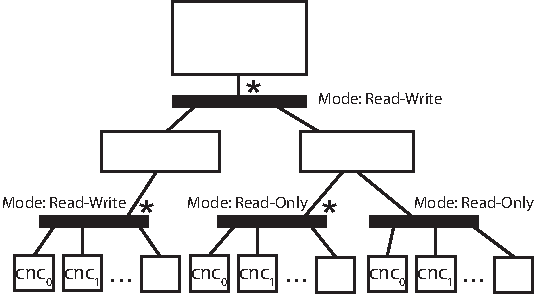
\includegraphics[scale=0.45]{figs/CNC_State.pdf}
\label{fig:depexamp:a}
}
\subfigure[{\tt distribute\_charge} depends on {\tt calc\_new\_currents}.]{ 
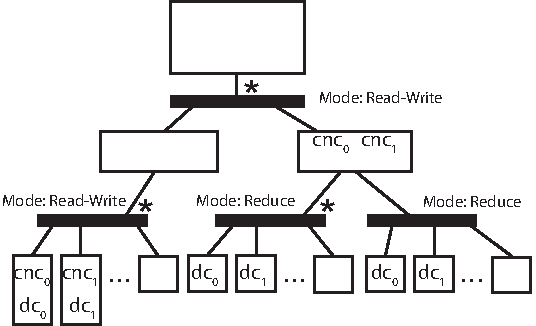
\includegraphics[scale=0.45]{figs/DC_state.pdf}
\label{fig:depexamp:b}
}
\subfigure[{\tt update\_voltages} depends on {\tt distribute\_charge}.]{
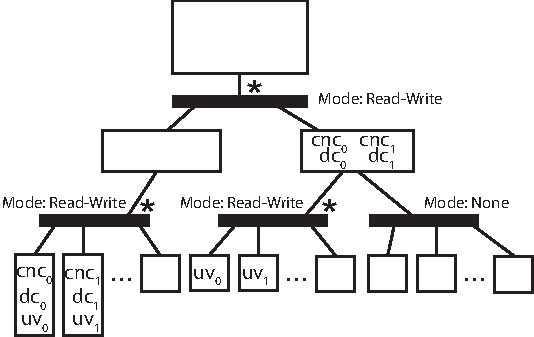
\includegraphics[scale=0.45]{figs/UV_State.pdf}
\label{fig:depexamp:c}
}
\subfigure[An {\tt update\_voltages} mapping.]{
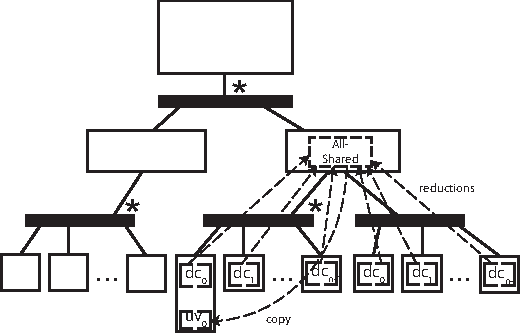
\includegraphics[scale=0.45]{figs/UV_Update.pdf}
\label{fig:depexamp:d}
}
\label{fig:depexamp}
\caption{Dependence analysis examples from {\tt circuit\_simulation}.}
\end{figure*}

There are two parts to this analysis:
the walk from a region root to $r'$ and the off-path work
to move dependent tasks to the least common ancestor on the path.
Clearly the walk to $r'$ is bounded by the depth of the region tree.
The off-path work can be made efficient by maintaining at each node a
record of which subtrees have tasks in them and with what privileges,
enabling the off-path search to traverse directly and only to
dependent tasks.  The off-path work is proportional to how far a task
is moved back up the region tree.  Thus, for each region argument a
task is initially placed at some depth in the tree and subsequently
only moved up towards the root, so the overall work per region is (amortized)
${\cal O}(d)$.  
%In practice, we have found this level of efficiency,
%where analyzing mapping dependences is linear in the number regions used (and not the square) and
%proportional to the depth of the region tree (and not its size)
%to be very important in minimizing the overhead of the SOOP.

We illustrate dependence analysis using the four tasks discussed
above.  Many more tasks are executed by the circuit simulation,
but this subset illustrates the important
points. Figure~\ref{fig:depexamp} shows the node region tree in three
stages.  In Figure~\ref{fig:depexamp:a}, the two tasks
{\tt calc\_new\_currents(pieces[0])} ($c_0$) and {\tt
    calc\_new\_currents(pieces[1])} ($c_1$) have been placed on their region arguments,
  which determines these two tasks are independent.
Next, in Figure~\ref{fig:depexamp:b}, the task {\tt distribute\_charge(pieces[0],dt)} ($d_0$)
has dependences with both $c_0$ and $c_1$ caused by aliasing between the pieces of the
shared node partition and the ghost node partition, so both $c_0$ and $c_1$ are moved to
the {\tt p\_nodes\_pvs[1]} region.  Finally, the task {\tt update\_voltages[1]} ($u_1$) causes
$d_0$ to also be moved to {\tt p\_nodes\_pvs[1]} for essentially the same reason; the final
state of the node region tree is shown in Figure~\ref{fig:depexamp:c}.


\subsection{Stage 2: Distribution}
\label{sec:dist}

The first step in distribution is that $t$ waits for all tasks on which $t$ depends to
map; nothing happens to $t$ during this time.  Once $t$'s mapping
dependences are satisfied, $t$ is ready to be mapped and is placed
in the mapping queue.

Once in the mapping queue, SOOPs on other processors in the system may
ask to steal $t$ from its home SOOP.  The home SOOP may decline the
request, but if the request is granted, task $t$ along with a copy of
$t$'s region forest is sent to the remote SOOP.  If $t$ has not been
stolen when it reaches the head of the queue, the SOOP decides whether
to execute $t$ on the local processor or send it to another processor.

Thus, task distribution to processors in Legion is both ``pull'' (stealing) and ``push''.
The various policies (whether steal requests are granted, when to send
a task to another processor, etc.) are part of the {\em mapping interface}
and can be defined by the user (see Section~\ref{sec:mapping}).


\subsection{Stage 3: Mapping}
\label{sec:map}

%After a processor $p$ is chosen for a task, $t$ executes entirely on $p$.
%nBefore execution, however, we must {\em map} $t$, i.e., choose the
%physical instances for $t$'s logical regions.  A physical instance is assigned
%to a particular memory in the machine and holds a snapshot of the region's data
%from some point in time; a {\em valid} physical instance has data that reflects
%all the updates of all previously mapped tasks.

The region tree is also used to hold mapping information.  Each logical region $r$ maintains a
list of its physical instances and which sibling tasks are using which
instances and with what permissions.  The important correctness
property established by stage 1 is that all
tasks which $t$ may depend on map before $t$ maps and no task that may depend on
$t$ maps before $t$ finishes mapping.  Thus, the region tree at the
moment $t$ maps contains a consistent view of what the state of memory
will be after $t$'s dependence predecessors execute.

There are two steps to mapping a region $r$ used by
task $t$.  First, the mapper must ensure there is at least one {\em valid}
physical instance of $r$ for $t$ to use.  If an instance of a subregion of $r$ has been written by a previous task,
for example, it is necessary to copy that subregion back to an instance of the parent $r$ so that $t$
sees the correct data. In the second step, the mapping interface selects one of the
valid physical instances of $r$ or creates a new one.  
We focus here on the first step; the mapping interface is discussed further in Section~\ref{sec:mapping}.

%For example, assume there is one physical instance $s$ of
%logical region $r$ and that a task $t'$ that mapped prior to $t$ is recorded as writing a
%physical instance $s_i$ of subregion $r_i$ of $r$.  At this point there
%is no valid instance of $r$, because $s$ does not include
%the updates to $s_i$.  To restore $s$ to a valid instance of $r$ the
%system must shedule an operation after $t'$ to copy
%$s_i$ back into $s$.  


%Typical
%policies are to to choose the existing physical instance that is
%closest to $t$'s processor, or to create a new instance (by issuing a
%copy operation) in the memory closest to $t$'s processor.


Detecting or creating a valid instance of $r$ is, at its core, a dependence analysis on
physical instances and thus similar to the mapping dependence analysis on logical
regions described in Section~\ref{sec:dep}.  Consider any task $t'$ using
physical instance $s'$ of logical region $r'$ in the region tree.  There are four cases.
\begin{enumerate}
\item If $t'$ has only read privileges
for $r'$ it cannot invalidate any instance of $r$.

\item If $t'$ has read/write privileges for $r'$, and $r$ aliases $r'$,
   then $s'$ must be copied to an instance $s''$ of
  $\lca{r}{r'}$ and a fresh instance of $r'$ created from $s''$.
%  (if either $r = \lca{r}{r'}$ or $r' = \lca{r}{r'}$ one of the two
%  copies is omitted)
Instance $s'$ is removed from the region tree
  but not deallocated (see Section~\ref{sec:clean}).

\item If $t'$ has reduce privileges for $r'$ and $t$ has reduce
  privileges for $r$ and both use the same reduction operator, then
  nothing is done.  This is the only case in which a writer
  does not require a valid instance---because reductions can be
  reordered, combining the instances of $r$ and $r'$ (if they
  alias) can be deferred to a later consumer of the data (see case
  4).

\item If $t'$ has reduce privilege for $r'$ and $t$ has read, write, 
  or reduce privileges with a different operator than $t'$
  for $r$, and $r$ aliases $r'$, then $s'$ must be
  reduced (using $t'$'s reduction operator) to an instance $s''$ of
  $\lca{r}{r'}$ and then a fresh instance of $r'$ created from $s''$.
%  (If $r' = \lca{r}{r'}$ the reduction is unneeded, and if $r =
%  \lca{r}{r'}$ the copy is unneeded.) 
Instance $s'$ is removed from the region
  tree but not deallocated.
\end{enumerate}

%Not all of these cases can occur simultaneously for a particular
%region argument $r$ of task $t$.  There may always be multiple
%previous readers (case 1), but the mapping dependence analysis
%guarantees that there would only be one previous writer (case 3) or
%one or more reducers (cases 2 and 4).  
To map $r$, we walk from $r$'s
root ancestor in the region forest to $r$, along the way exploring
off-path subtrees to find region instances satisfying cases 3 and
4. The details and analysis are similar to the implementation of dependence
analysis in Section~\ref{sec:dep}; the amortized work per region mapped
is proportional to the depth of the region tree.

As part of the walk any required copy and reduction operations are
issued to construct a valid instance of $r$.  These operations are
deferred, waiting to execute on the tasks that produce the data they
copy or reduce. Similarly, the start of $t$'s execution is made
dependent on completion of the copies/reductions that construct the
instance of $r$ it will use.

Figure~\ref{fig:depexamp:d} shows part of the mapping of task {\tt update\_voltages[0]}; we focus
only on the shared nodes.
Because the immediately preceding {\tt distribute\_charges} tasks all performed the same reduction
on the shared and ghost nodes they were allowed to run in parallel.  But {\tt update\_voltages[0]}
needs read/write privilege for {\tt pieces[0].rn\_shr}, which forces all of the reductions to be merged
back to an instance of the {\tt all-shared} nodes region, from which a new instance of {\tt pieces[0].rn\_shr} is copied and used by {\tt update\_voltages[0]}.

Figure~\ref{fig:gpumapping} shows a timeline of our mapping of the
circuit simulation on a cluster of GPUs.  The $i$th private node and
wire regions are mapped to the $i$th GPU's DRAM and simply left there
for all three phases of the simulation.  The $i$th shared and ghost
regions are mapped to zero-copy memory most of the time, but, as just
illustrated, must be reduced out to the all-shared node region in the
global (GASNet) memory and then a new instance of the shared
subregions created with the updated information before the {\tt
  update\_voltages} tasks execute.  A similar situation arises before
{\tt calc\_new\_currents} tasks run again: the updates to the shared
nodes by {\tt update\_voltage} must be propagated to the ghost nodes
before continuing.

\begin{figure}
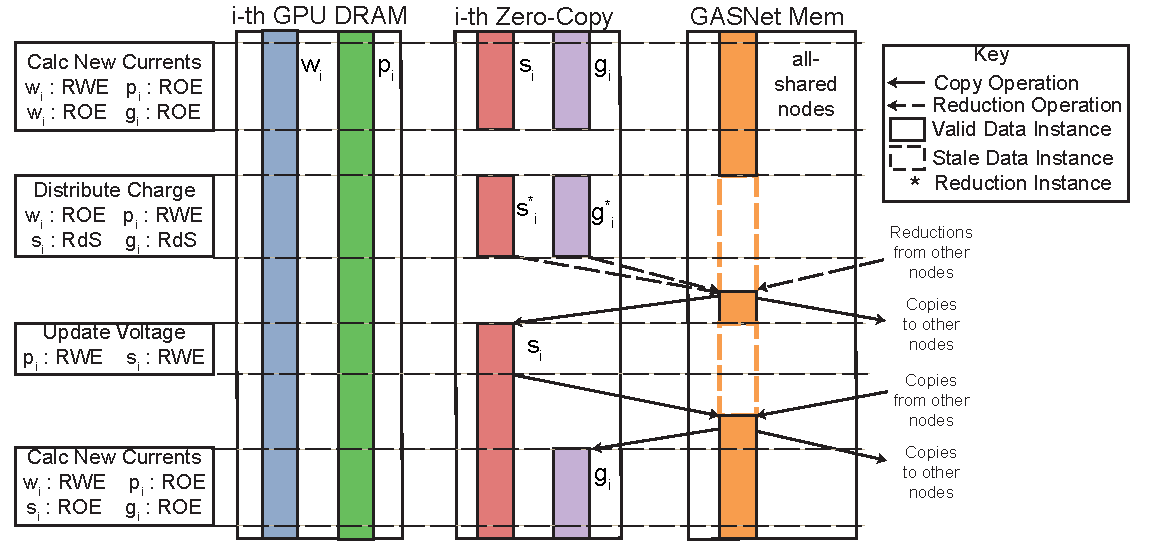
\includegraphics[scale=0.48]{figs/CircuitMem.pdf}
\caption{Tasks and data for the circuit simulation on a cluster of GPUs.}
\label{fig:gpumapping}
\end{figure}

\subsection{Stage 4: Execution}
\label{sec:exec}

Once a task $t$ has been mapped it enters the execution stage of the SOOP.  When all of
the operations (other tasks and copies) on which $t$ depends have completed, $t$ is
launched on the processor.  When $t$ spawns subtasks, they are recursively scheduled as siblings by
the SOOP using $t$ as the parent task and $t$'s region arguments as the roots of the region forest.


\subsection{Stage 5: Clean-Up}
\label{sec:clean}

Once task $t$ is done executing its state can be reclaimed Dependence
and mapping information is removed from the region tree (it can
usually be removed even earlier).  The most involved aspect of
clean-up is collecting physical instances that are no longer in use,
for which we use a distributed reference counting scheme.


